\documentclass[onlytextwidth]{beamer}
\usepackage[utf8]{inputenc}
\usepackage{microtype}
\usepackage{amsmath}
\usepackage{amssymb}
\usepackage[nomessages]{fp} %\FPeval{\var-name}{2*sin(pi/6)}
\usepackage{siunitx} %units in math. eg 20\milli\meter
\usepackage{yhmath} % for arcs, overparenth command
\usepackage{tikz} %graphics
\usetikzlibrary{quotes, angles}
%\usepackage{graphicx} already loaded by beamer class
%consider setting \graphicspath{{images/}}
%\parskip ?? to avoid paragraph indent
\usepackage{multicol} %may not need this package, just columns environment
\usepackage{venndiagram}

\subtitle[BECA]{Bronx Early College Academy}
\author[Huson]{Christopher J. Huson PhD}

\setbeamertemplate{headline}{\vskip2mm 
  BECA / \insertshortauthor \, / \inserttitle
  \hfill 
  \insertsection
  }

\title{Routines and Expectations}
\date{2022-2023}

\begin{document}
\frame{\titlepage}

\section[Outline]{}
\frame{\tableofcontents}

\section{1.1 1st day of Geometry, Segment addition, 13-14 Sept}
\frame
{
  \frametitle{Learning Target: I can measure and diagram my world}
  \framesubtitle{CCSS: HSG.CO.A.1 Know precise geometric definitions \hfill \alert{1.1 Tuesday 13-14 Sept}}

  Welcome back to school
  \begin{block}{Expectations}
  \begin{enumerate}
      \item Notebook first page: Name / Course / Instructor
      \item Practice: pocket folder
      \item Tools: calculator, ruler, Chromebook (charged), paper/pencil/pen
  \end{enumerate}
  \end{block}
  Supply list: Composition book, looseleaf, pencils \& pens, \\*
  compass and ruler, calculator; Optional: folder \\[0.25cm]
  Homework: Write for me your ``math autobiography''
}

\frame
{
  \frametitle{Take class notes in a composition book}
  \begin{block}{Use this notebook format (required)}
    \begin{enumerate}
      \item In the front, write your name, my contact info, your passwords
      \item Each page in the top left corner: \\ \qquad First+Last Name \\
      \qquad 14 September 2021 \\ \qquad Learning Target: I can measure and diagram my world \vspace{0.25cm}
      \item Copy definitions using your own words
      \item Write down example diagrams and problems
    \end{enumerate}
    \end{block}
}

\frame
{
  \frametitle{Casio fx-9750GII calculator - due Friday 1 October}
  \begin{multicols}{2}
  In the high school at BECA we use the Casio fx-9750GII.\\[5pt] 
  It is allowed on the Regents exams, SAT tests, and International Baccalaureate exams.\\[5pt]
  You may use a different calculator in Geometry if you prefer, but I recommend buying the Casio fx-9750GII.\\[5pt]
  (see me if buying a calculator is a hardship for your family)
  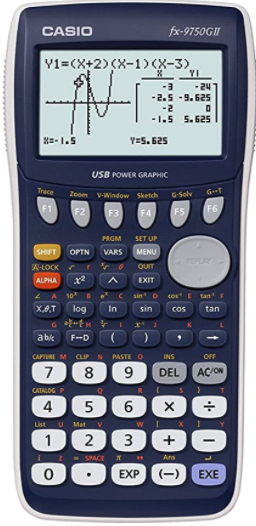
\includegraphics[width=3.5cm]{casio_fx-9750GII.png}
  \end{multicols}
}

\end{document}